\documentclass{standalone}
\usepackage{hsbcommon}
\begin{document}
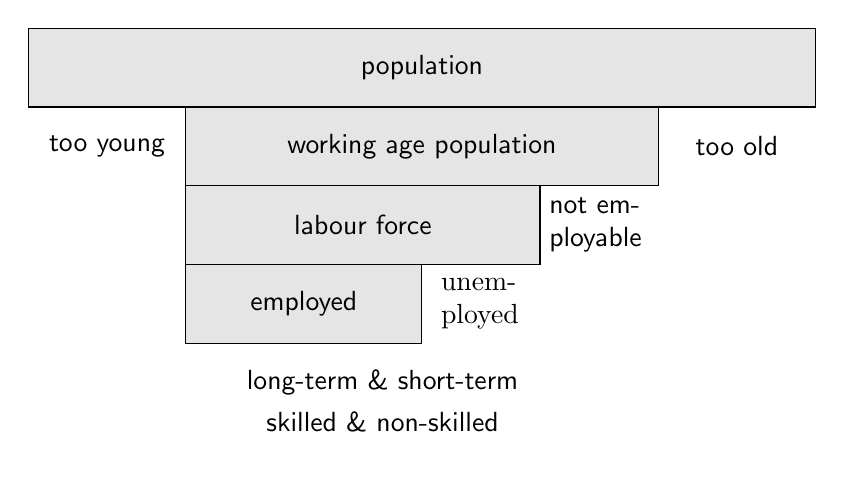
\begin{tikzpicture}
    \tikzset{
        myboxed/.style={
                draw,
                minimum height=1cm,
                anchor=west,
                fill=gray!20,
                font=\sffamily
            },
        unboxed/.style={
                minimum height=1cm,
                anchor=west,
                font=\sffamily
            }
        }
    \node[myboxed,minimum width=10cm] at (0,0) {population};
    \node[myboxed,minimum width=6cm] at (2,-1) {working age population};
        \node[unboxed,minimum width=2cm] at (0,-1) {too young};
        % \node[unboxed,text width=2cm] at (0,-1.5) {in education};
        \node[unboxed,minimum width=2cm] at (8,-1) {too old};
    \node[myboxed,minimum width=4.5cm] at (2,-2) {labour force};
        \node[unboxed,text width=1.5cm] at (6.5,-2) {not employable};
    \node[myboxed,minimum width=3cm] at (2,-3) {employed};
        \node[text width=1.5cm] at (6,-3) {un\-em\-ployed};
    \node[unboxed,minimum width=5cm] at (2,-4) {long-term \& short-term};
    \node[unboxed,minimum width=5cm] at (2,-4.5) {skilled \& non-skilled};
    
    
\end{tikzpicture}
\end{document}